\section{Experiments}\label{sec:experiments}
Sections~\ref{sec:new-sim} and~\ref{sec:credit} report new experiments that run the gate. Section~\ref{sec:carried} reports how large the pooled excess is on the same register and what knowledge produces it; its first table is carried over from \cite{mahomane2026}, and the floors that follow are new.

\subsection{Toy audit: optional monitoring and adaptive registration}\label{sec:new-sim}
We first ran the gate on known Bernoulli laws, where Assumption~\ref{ass:law} holds by construction. One coordinate has weight $w=1/8$, family error $\alpha=0.05$, tolerance $\tau=0.12$ and fixed bet $q=0.03$, so the threshold is $1/(\alpha w)=160$ and the coordinate's own false-certification bound is $\alpha w=0.00625$. Each of 2,000 replications draws at most 300 attacks, from a safe law with success probability 0.04 or from the null boundary at 0.12. The comparator is a one-sided Clopper--Pearson test at level $\alpha w$ applied once, after draw 300. Table~\ref{tab:new-audit} gives the results (seed 2709).

\begin{table}[t]\centering\small
\caption{Toy audit, 2,000 replications per law. ``Gate'' monitors every draw up to 300; ``fixed CP'' tests once after draw 300. Monte Carlo standard errors in brackets.}\label{tab:new-audit}
\begin{tabular}{lrrr}
\toprule
True success probability & Gate certifies & Fixed CP certifies & Median draws to certify\\\midrule
0.04 (safe) & 0.9560 (0.0046) & 0.9990 (0.0007) & 98\\
0.12 (null boundary) & 0.0050 (0.0016) & 0.0055 (0.0017) & 75$^\ast$\\\bottomrule
\end{tabular}\\[2pt]
\parbox{.92\linewidth}{\footnotesize $^\ast$Median over the ten false certifications; not an expected certification time.}
\end{table}

At the null boundary the gate certified falsely in 10 of 2,000 runs, a rate of 0.0050 with standard error 0.0016, below the coordinate's bound of 0.00625 and far below the family budget $\alpha=0.05$. Under the safe law the gate certified less often than the fixed test (0.9560 against 0.9990), and it did so after a median of 98 draws rather than 300.

In a second run, a null-boundary coordinate was registered only after an independent safe coordinate had been certified; this happened in 1,902 of 2,000 runs. The null coordinate certified falsely in 10 of the 2,000 runs, an overall rate of 0.0050 (standard error 0.0016), against its bound of 0.00625 and the family budget of 0.05. Because the two streams are independent, the registration rule does not change the law of the null stream, and this rate is another estimate of the single-coordinate rate. This run goes through the shipped gate implementation, which registers the second coordinate only after the first has certified; it checks the implementation, and it does not test the theorem under bets or targets that depend on the past.

\subsection{Choosing a floor on a synthetic credit register}\label{sec:credit}
\paragraph{Register and attacks.} The synthetic register runs over six monthly vintages. Its first vintage publishes 27{,}167 loans with no suppression. About four per cent of loans leave each month and do not return, and a similar number of new loans enter, so the stock is close to constant and 81 per cent of the loans in the first vintage are live in all six. A loan's key (region, sector and size class) and exposure do not change between vintages. Each release publishes, for every loan it contains, a loan pseudonym that is the same in every vintage, the key and the exposure. A policy deletes every loan in a key cell holding fewer than $k$ loans. The adversary follows Assumption~\ref{ass:threat}: it knows the target's key, restricts attention to released loans in the target's key cell, and names the loan with the largest posterior given its exposure readings; ties are broken at random. When it knows the target's history it also requires a candidate's pattern of appearances across the vintages to match the target's, in both directions. We declare three adversaries before the audit: one release and one reading; six vintages, one reading and the history; and six vintages, a reading per live vintage and the history. Targets are drawn with replacement from the loans in the first release.

\paragraph{Design.} The main design is a release chain (Proposition~\ref{prop:release}) over the floors $k=300$, 200, 150, 100, 75, 50, 40, 30, 20, 15, 10, 5 and 1, audited in that order. At each floor the three coordinates are audited on fresh targets, at most 3{,}000 each, at the full threshold $1/\alpha=20$; the floor passes only if all three certify, and the chain stops at the first floor that fails. The bet is $\min\{(Y+1/2)/(B+1),\,0.11\}$ from earlier draws of the same coordinate. Five other designs receive the same draws: one chain per attack at $\alpha/3$, which is the price of choosing the adversary after the audit; the gate with all 39 coordinates registered at the start, stopped at the first failing floor; fixed-sequence Clopper--Pearson intersection-union tests at level $\alpha$ with 3{,}000 and with 1{,}000 attacks per coordinate; and Clopper--Pearson looks every 500 attacks with $\alpha$ split over the six looks. The true risk of each coordinate was estimated from a separate draw of 100{,}000 targets, and the true floor is the last level, from the top, at which all three estimated risks lie below the tolerance. We ran 20 attack streams on one register. Because 20 streams cannot test an error rate of 0.05, validity was checked separately: the release chain was run 400 times on Bernoulli streams at the estimated risks, and again with every risk raised by 0.01 and by 0.02.

\begin{table}[t]
\centering
\caption{Choosing the cell-count floor on the synthetic credit register over 20 attack streams, tolerance 0.12, $\alpha=0.05$. The agency declares three attacks before the audit (one release with one reading; six releases with one reading and the loan's history; six releases with a reading per live vintage and the history), and a floor passes only when all three meet the tolerance. Each design audits the floors from 300 down and stops at the first that fails. Entries give each floor chosen with the number of streams in brackets, and the median total number of attacks. The estimated true floor uses 100{,}000 separate targets per coordinate. All designs see the same draws.}
\label{tab:chain-audit}
\small
\begin{tabular}{lrr}
\toprule
Design & Floor chosen & Attacks \\
\midrule
Estimated true floor & 100 & -- \\
\midrule
Gate, release chain at $\alpha$ & 100 (1), 150 (19) & 6{,}422 \\
Gate, one chain per attack at $\alpha/3$ & 150 (20) & 13{,}764 \\
Gate, all 39 registered at the start & 150 (19), 200 (1) & 9{,}002 \\
Fixed sequence, 3{,}000 per coordinate & 100 (4), 150 (16) & 36{,}000 \\
Fixed sequence, 1{,}000 per coordinate & 100 (2), 150 (15), 200 (3) & 12{,}000 \\
Looks every 500, Bonferroni over looks & 100 (3), 150 (17) & 10{,}000 \\
\bottomrule
\end{tabular}
\end{table}


\paragraph{Results.} Table~\ref{tab:chain-audit} gives the results. Each row is one design run on the same 20 attack streams; the middle column lists the floors it chose, with the number of streams in brackets, and the last column is the median number of attacks it spent. The first row is the benchmark: the floor that the estimated true risks imply. The estimated true floor is 100, set by the full pooled attack, whose risk is 0.116 at $k=100$, 0.133 at 75 and 0.091 at 150. The release chain chose 150 in 19 streams and 100 in one, using a median of 6{,}422 attacks; no design chose an unsafe floor. On Bernoulli streams at the estimated risks the release chain chose an unsafe floor in none of 400 runs; with every risk raised by 0.01 it did so in 6 (a rate of 0.015), and with every risk raised by 0.02 in none, because the chain then stops at stricter floors. The floor of 150 keeps 5{,}553 of 27{,}167 loans.

\paragraph{Audit length.} Proposition~\ref{prop:length} explains why the chain seldom chose 100. At $k=100$ the full pooled risk of 0.116 lies above the cap of 0.11 on the bet, so the capped bet has negative drift and certifies only by chance, as it did in one stream, and even the best fixed bet would need about 43{,}000 draws on average. At $k=150$, with risk 0.091, the bound is about 720 draws. A cap closer to the tolerance would certify more near-boundary floors at a large cost in attacks; the design choice is between that cost and a stricter floor.

\subsection{A neural network in the loop}\label{sec:neural-run}
Figure~\ref{fig:neural-pipeline} shows how a network enters the audit without entering the error bound. The three declared attacks were first run on 25 floors with 400 development targets each, on seeds the final audit never uses. A network with two hidden layers of 16 units, one output per attack, was fitted to these counts by the binomial likelihood, with a third of the floors held out for early stopping, and a logistic model was fitted to the same counts. Its inputs are features of a floor that need no attack: the floor, the share of loans kept, the mean released cell size and the share of released loans not live in every vintage. Before any final outcome was drawn, each model's predictions were frozen as a plan: the bet for every coordinate, $\min\{\hat r,0.11\}$, and a start floor one step stricter than the floor the model predicted to be safe. The release chain then audited each plan on the same final draws as Table~\ref{tab:chain-audit}, with a fifth of the budget held in reserve for a second chain from $k=300$ if the first failed at its start.

\begin{figure}[t]
\centering
\begin{tikzpicture}[font=\small,node distance=0.5cm and 1.8cm,
  stage/.style={draw,rounded corners=2pt,align=center,text width=2.8cm,minimum height=1.1cm},
  dev/.style={stage,fill=gray!15},
  final/.style={stage,pattern=north east lines,pattern color=gray!40},
  frozen/.style={stage,double,double distance=1.2pt},
  >=Stealth]
  \node[dev] (a) {1. Development\\attacks on a dense\\floor grid, own seeds};
  \node[dev,right=of a] (b) {2. Network fitted by\\binomial likelihood\\(logistic baseline)};
  \node[frozen,right=of b] (c) {3. Frozen plan\\bets and start floor,\\with its digest};
  \node[final,below=1.3cm of c] (d) {4. Release chain\\on fresh targets};
  \node[stage,left=of d] (e) {Floor certified,\\or none};
  \node[stage,left=of e] (f) {Reserve chain\\from $k=300$ if the\\first floor fails};
  \draw[->] (a) -- node[above,font=\scriptsize]{counts} (b);
  \draw[->] (b) -- node[below,font=\scriptsize]{predictions} (c);
  \draw[->] (c) -- node[right,font=\scriptsize]{fixed before outcomes} (d);
  \draw[->] (d) -- (e);
  \draw[->,dashed] (d.south) -- ++(0,-0.5) -| node[near end,left,font=\scriptsize]{first floor fails} (f.south);
  \draw[->,dashed] (f) -- (e);
  \draw[densely dotted,thick] ($(a.north west)+(-0.25,0.35)$) rectangle ($(b.south east)+(0.25,-0.35)$);
  \node[anchor=south west,font=\scriptsize] at ($(a.north west)+(-0.25,0.35)$) {development evidence only};
\end{tikzpicture}
\caption{The neural release pipeline. Grey boxes use development attacks only;
the double box is the plan, frozen with its digest before any final outcome
exists; the hatched box is the only stage whose outcomes can certify a floor. The
network's predictions choose the bets and the floor at which the release chain
starts, so a poor network costs attacks but cannot raise the chance of certifying
an unsafe floor.}
\label{fig:neural-pipeline}
\end{figure}

\begin{table}[t]
\centering
\caption{The neural release pipeline on the synthetic credit register, 20 attack streams, tolerance 0.12, $\alpha=0.05$. Every design is a release chain over the three declared attacks on the same final draws; they differ only in where the bets and the start floor come from. The network and the logistic model are fitted to development attacks on separate seeds and fixed before the final audit. Entries give each floor chosen with the number of streams in brackets, and the median number of attacks.}
\label{tab:neural-pipeline}
\small
\begin{tabular}{lrr}
\toprule
Source of bets and start & Floor chosen & Attacks \\
\midrule
Running-rate bets, chain from 300 & 100 (1), 150 (19) & 6{,}422 \\
Logistic bets, chain from 300 & 100 (2), 150 (18) & 5{,}572 \\
Network bets, chain from 300 & 100 (2), 150 (18) & 5{,}620 \\
Logistic bets and start floor & 100 (1), 150 (19) & 5{,}019 \\
Network bets and start floor & 100 (1), 150 (19) & 5{,}044 \\
\bottomrule
\end{tabular}
\end{table}


Table~\ref{tab:neural-pipeline} gives the results. The first row repeats the release chain of Table~\ref{tab:chain-audit}. All five designs chose 150 in 18 or 19 of the 20 streams and none chose an unsafe floor, as Theorem~\ref{thm:gate} and Proposition~\ref{prop:release} require whatever the quality of the predictions. The network's bets cut the median number of attacks from 6{,}422 to 5{,}620, and its bets and start floor together to 5{,}044, about a fifth fewer; the reserve was never used. The logistic model did as well, and its predictions were closer to the estimated true risks (mean absolute error 0.004 against 0.008). On this register the saving comes from using development evidence for the bets and the start, not from the depth of the model. The network is the default in the software because it extends to many more features and declared attacks; the logistic model is reported beside it so that the comparison stays visible.

Figure~\ref{fig:neural-predictions} shows the predictions themselves. Fitted only to the development rates (crosses), the network's frozen predictions (solid line) follow the true risks (dotted line) for all three attacks and cross the tolerance near $k=100$ for the full pooled attack, where the estimated true floor lies. Table~\ref{tab:neural-fit} gives the fit: the two models reach almost the same held-out log loss (0.3482 and 0.3480), both predict a floor of 100 and start the chain at 150, and the network's mean error against the true risks (0.008) is twice the logistic model's (0.004), because it follows more of the scatter in the development rates.

\begin{figure}[t]
\centering
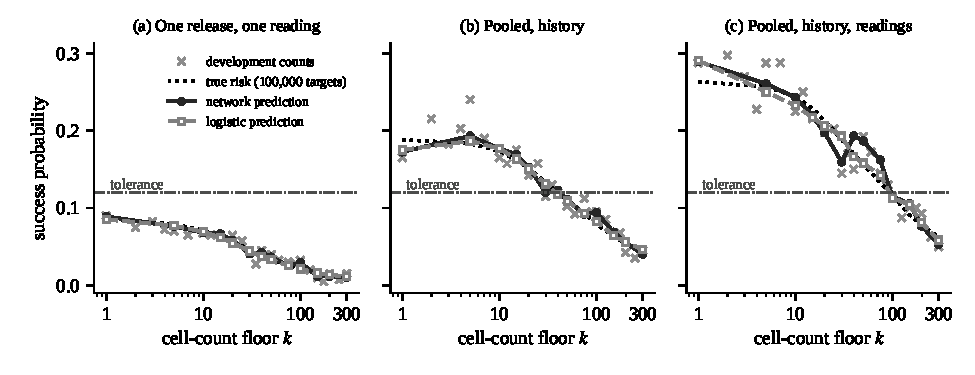
\includegraphics[width=\linewidth]{figures/fig_neural_predictions.pdf}
\caption{What the neural network predicted. For each declared attack, the frozen
predictions of the network (solid line, filled circles) and of the logistic model
(dashed line, open squares) against the true risk estimated from 100{,}000
separate targets (dotted line), with the development success rates the models were
fitted to (crosses, 400 targets each) and the tolerance (dash-dot line). The
network was fitted to the crosses alone and never saw the final audit.}
\label{fig:neural-predictions}
\end{figure}

\begin{table}[t]
\centering
\caption{What the two models learned from the development attacks. Log losses are the binomial log loss per development attack on the training and held-out floors; the epoch is where held-out loss was lowest. Errors compare each model's frozen prediction with the true risk, estimated from 100{,}000 separate targets, over the 39 coordinates of the release grid. The predicted floor is the last floor, from $k=300$ down, at which every predicted risk lies below the tolerance; the start floor is one step stricter.}
\label{tab:neural-fit}
\small\setlength{\tabcolsep}{4pt}
\begin{tabular}{lrrrrrrr}
\toprule
 & \multicolumn{2}{c}{Log loss} & & \multicolumn{2}{c}{Error against truth} & \multicolumn{2}{c}{Floor}\\
\cmidrule(lr){2-3}\cmidrule(lr){5-6}\cmidrule(lr){7-8}
Model & Training & Held out & Epoch & Mean & Largest & Predicted & Start \\
\midrule
Network, two hidden layers & 0.3240 & 0.3482 & 1146 & 0.008 & 0.031 & 100 & 150 \\
Logistic model & 0.3245 & 0.3480 & 2067 & 0.004 & 0.027 & 100 & 150 \\
\bottomrule
\end{tabular}
\end{table}


\subsection{What produces the pooled excess}\label{sec:carried}
In a synthetic population of 200,000 units with a five per cent release sample, four releases that are each 3-anonymous, joined through a persistent pseudonym, have single-release identification probabilities summing to 0.2530, which bounds the chance that some single release succeeds by~\eqref{eq:union}; the pooled attack succeeds with probability 0.4581. On four 3-anonymous variants of a public Census sample of 29,501 records, joined the same way, the corresponding figures are 0.381 and 0.709. These figures are carried over from \cite{mahomane2026}; the credit-register results below are new.

\begin{table}[t]\centering\small
\caption{Share of 4,000 targets named correctly on the synthetic credit register, with the exact one-sided 95 per cent upper bound in brackets. The middle columns change one factor at a time on the same targets; every pooled column assumes the adversary knows the target's history.}\label{tab:carried}
\begin{tabular}{lrcccc}
\toprule
 & & \multicolumn{2}{c}{One release} & \multicolumn{2}{c}{All six releases}\\\cmidrule(lr){3-4}\cmidrule(lr){5-6}
Policy & Kept & One reading & Six readings & One reading & Six readings\\\midrule
No suppression & 27{,}167 & 0.089 (0.097) & 0.158 (0.168) & 0.191 (0.201) & 0.260 (0.272)\\
$k=5$ & 26{,}885 & 0.074 (0.081) & 0.141 (0.150) & 0.183 (0.194) & 0.269 (0.281)\\
$k=10$ & 26{,}019 & 0.070 (0.076) & 0.130 (0.139) & 0.179 (0.190) & 0.244 (0.256)\\\bottomrule
\end{tabular}
\end{table}

Table~\ref{tab:carried} splits the pooled excess. With no suppression, one release and one reading give 0.089 and the full pooled attack 0.260. Six readings in one release give 0.158, and pooling with one reading gives 0.191: the target's history is worth more than five further readings. Pooling works through the history: a candidate whose pattern of appearances differs from the target's is excluded, and the 19 per cent of loans that are not live in every vintage are nearly always found.

\begingroup\let\small\footnotesize\begin{table}[t]
\centering
\caption{What sets the programme floor on the synthetic credit register, tolerance 0.12. History: the adversary knows in which vintages the target's loan is live. The floor is chosen by fixed-sequence testing from $k=300$ down on one draw of 4{,}000 targets and confirmed on a second, independent draw (rate, with exact 95 per cent upper bound); where confirmation fails the next stricter level that passes is shown. Loans and exposure are the percentages of the first release kept at that floor. The subgroup floor requires every size class to meet the tolerance, with the largest firms on a stratified draw, from $k=200$ down. The insider reads exposure with error 0.01 on the log scale. In the Floor column ``none'' means no level up to 300 passes, and in the Subgroup column no level up to 200.}
\label{tab:robust}
\small\setlength{\tabcolsep}{3pt}
\begin{tabular}{lrrrrr}
\toprule
Adversary & Floor & Confirmation & Loans (\%) & Exposure (\%) & Subgroup \\
\midrule
One release, one reading & 1 & 0.084 (0.092) & 100 & 100 & 20 \\
Six releases, one reading, no history & 1 & 0.083 (0.091) & 100 & 100 & -- \\
Six releases, one reading, history & 75 & 0.096 (0.104) & 45 & 11 & 200 \\
Six releases, reading per vintage, no history & 20 & 0.105 (0.114) & 85 & 52 & -- \\
Six releases, reading per vintage, history & 150 & 0.101 (0.109) & 20 & 4 & none \\
Insider: exact exposure, history & none & -- & -- & -- & -- \\
\midrule
\multicolumn{6}{l}{\emph{Exposure published to one significant figure}}\\
One release, one reading & 1 & 0.079 (0.086) & 100 & 100 & -- \\
Six releases, one reading, history & 50 & 0.111 (0.119) & 58 & 20 & -- \\
Six releases, reading per vintage, history & 150 & 0.085 (0.092) & 20 & 4 & -- \\
Insider: exact exposure, history & none & -- & -- & -- & -- \\
\bottomrule
\end{tabular}
\end{table}
\endgroup

Table~\ref{tab:robust} (\nolinkurl{scripts/programme_robustness.py}) chooses the floor for each piece of the adversary's knowledge by fixed-sequence testing from $k=300$ down on one draw of 4{,}000 targets and confirms it on a second. Per release the floor is 1. Six vintages and one reading without the history also give 1; that is a property of the generator, in which published values never change. With the history the selection draw passed $k=50$, but the confirmation draw did not (upper bound 0.123), so the floor is the next stricter level, 75. With a reading per live vintage as well it is 150. Requiring every size class to meet the tolerance gives 20 for a single release and 200 for pooling with the history, and no level up to 200 passes for the full attack. An insider who knows exposure to within one per cent and knows the history defeats every floor up to 300, where it still names 42 per cent of targets. Publishing exposure to one significant figure hardly moves the outsiders' floors, since their readings are noisier than the rounding, but it halves the insider's success (0.388 against 0.772 with no suppression) and cuts the share of loans that published fields alone can relink across vintages from 1.00 to 0.10, which is what would make rotating pseudonyms worth doing. The floors keep little of the file: 75 keeps 45 per cent of loans and 11 per cent of exposure, and 150 keeps 20 and 4 per cent, with no large-firm loans. Table~\ref{tab:tolerance-floors} repeats the selection at tolerances of 0.05, 0.09 and 0.20, from the same draw. It reports the selection floor before confirmation, which is why pooling with the history shows 50 at 0.12 rather than the confirmed 75. The floors move by an order of magnitude across this range: at 0.05 a single release already needs 40 and the full attack has no floor up to 300, while at 0.20 the three outside attacks need 1, 5 and 30. Over 20 independent register draws at the declared reading noise the floors were 1, 40 to 75, and 100 to 150 (Supplement, Section~\ref{S-sec:s-methods}).

\begin{table}[t]
\centering
\caption{The floor chosen at four tolerances by the selection draw of Table~\ref{tab:robust}, before confirmation; at 0.12 pooling with the history therefore shows 50, where Table~\ref{tab:robust} shows the confirmed 75. ``None'' means no level up to 300 passes.}
\label{tab:tolerance-floors}
\small
\begin{tabular}{lrrrr}
\toprule
Tolerance & One release & Pooling, history & Full pooled & Insider \\
\midrule
0.05 & 40 & 300 & none & none \\
0.09 & 5 & 100 & 200 & none \\
0.12 & 1 & 50 & 150 & none \\
0.20 & 1 & 5 & 30 & none \\
\bottomrule
\end{tabular}
\end{table}

